\chapter{Design Flow}
\label{sec:design-flow}

In this chapter we introduce a novel design flow for creating
high-performance dataflow designs starting from C/C++ applications. We
explain the motivation and requirements for the proposed approach and
provide an overview of its three main components:
\begin{itemize}
\item the \emph{\FAST{} language}, used to express dataflow kernels
\item the \emph{aspect description repository} and \emph{weaver}, which group
  and apply the optimisation and transformation strategies encapsulate
  through aspects
\item the \emph{compilation backend}, used to generate FPGA bitstreams
  from dataflow designs and link the host code run-time
  application
\end{itemize}
We show how these three components can be integrated to produce an
automated design technique. We analyse the steps required to produce
an optimised design using the proposed approach and compare this with
alternative approaches using other start-of-the-art
technologies. Finally, we present an extension to our original
design-flow to support run-time reconfiguration.

\begin{comment}
\section{Overview}

Figure \ref{fig:design-flow-overview} provides a brief overview of the
proposed design flow. First a high level application is produced as
the input to our flow. This is then partitioned into a software part
and a hardware part to run on the dataflow accelerator. A dataflow
kernel is generated from the original description. Aspect descriptions
are used to control the optimisation process.

Thus the inputs to the design flow are:
\begin{itemize}
\item High-level source specification
\item Aspect descriptions for controlling the compilation process
\end{itemize}

\begin{figure}[!h]
  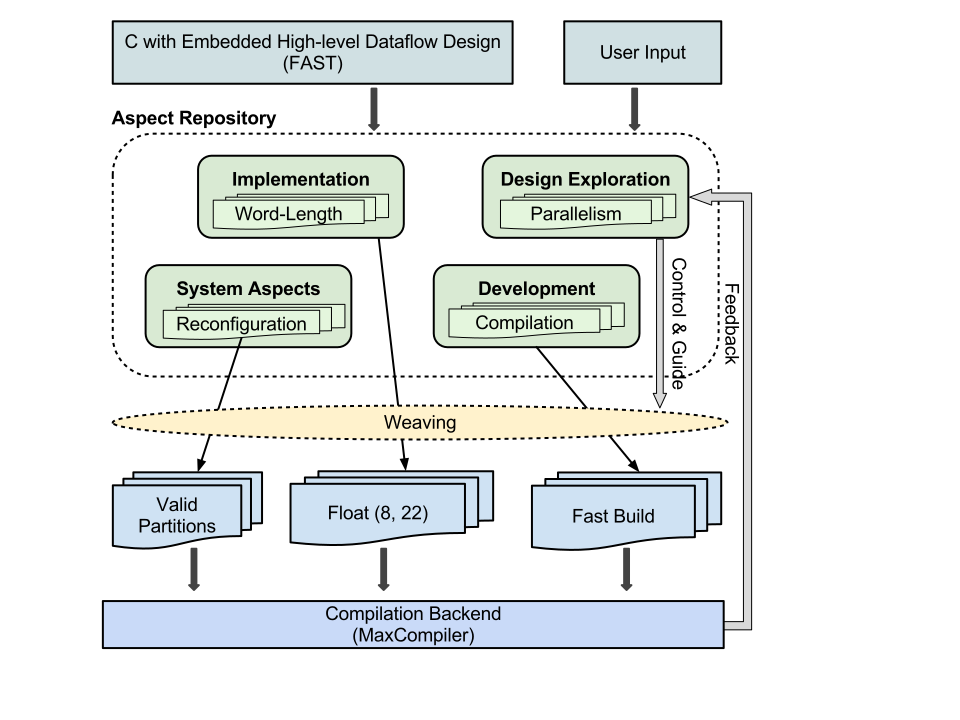
\includegraphics[scale=0.5, trim=60 50 0 0]{figs/asap13-design-flow.pdf_tex}
  \caption{Proposed approach for aspect-driven compilation of dataflow
    designs.}
  \label{fig:design-flow-overview}
\end{figure}

The design flow produces as its output a number of implementations based on
requirements specified through aspects.

The following algorithm describes the operation of the proposed design flow:

\begin{lstlisting}
  for (in as do als)
\end{lstlisting}
\end{comment}

\section{Design Goals}

Our design flow aims to improve both \emph{efficiency} (in terms of
performance and energy consumption) and \emph{productivity}. The
former is crucial to High Performance Computing, the latter helps
reduce development cost and time and is a well-known issue with
existing FPGA based acceleration solutions \cite{jones2010gpu}. To
achieve this we focus on maintaining or improving the
\emph{performance} and \emph{energy efficiency} of existing
applications while using a more systematic approach for design
optimisation that results in more \emph{portable} application code,
improves \emph{integration} with existing applications and
\emph{automate} time consuming and error-prone tasks that need to be
performed manually using traditional tools.

\subsection{Performance and Energy Efficiency}
When targeting HPC applications it is crucial that our design flow
results in high-performance, highly efficient designs. By analysing
existing implementations for advanced high-performance applications
such as Reverse Time Migration (\Cref{app:rtm-kernel}), we identify key
requirements of these designs:

\begin{itemize}

\item \textbf{Computation is the most significant part} of
  high-performance applications. For stencil computations this is
  usually a fairly large stencil operation over a large number of
  adjacent data-points (multiple points in each dimension). For
  example, the RTM kernel uses two stencil operations of 31 floating
  point additions, 18 floating point multiplications and 1
  subtraction (\Cref{app:rtm-kernel}, Lines \ref{app:rtmk-op1} and
  \ref{app:rtmk-op2}).  Additionally, these are replicated
  \texttt{Par} times (with Par as large as 12) which leads to a total
  of $((31 + 18 + 1) * 2 * 12) = 1200 $ floating point operations to
  be executed on each kernel cycle (in reality floating point
  operations are pipelined across 13 kernel cycles, but this is,
  generally, transparent to the user). Hence, our approach must
  provide a clear and concise manner to express computation
  (preferably standard operators).

\item Another crucial aspect in achieving high-performance is
  \textbf{replicating the design} across the chip to maximise speedup
  subject to maximum available bandwidth. This makes use of FPGA cache
  (around 4MB of fast-local memory) to reuse data across time
  steps. This pipeline replication is achieved through design
  parametrisation and loops whose bounds are known at
  compile-time. The parameters that indicate the replication factor are
  shared across the compute and memory kernels but also across the CPU
  code.

\item High-performance designs \textbf{maximise usage of on-board
    DRAM}. Especially for stencil type computations where a number of
  time step iterations are performed over the original data, it is
  crucial to have the data available in the large, high bandwidth
  on-board DRAM rather than on the CPU side. Bandwidth of the on-board
  DRAM is 40GB/s compared to 2GB/s over PCI-Express to CPU. However,
  supporting DRAM introduces the additional complexity of managing
  multiple kernels (since memory read and write commands are,
  preferably, generated from kernels separated from the original
  dataflow kernel -- see \Cref{app:mem-read-kernel})
  and. Additionally, special API calls for generating the read/write
  commands have to be supported (\Cref{app:mem-read-kernel}, Line
  \ref{app:memrk-dram}).

\item \textbf{Expose optimisation opportunities for backend
  tools}. For example, our MaxCompiler backend supports some degree of
  trade-offs when mapping computation to DSPs. Additionally various
  trade-offs can be achieved by disabling pipeline depth etc.  These
  optimisations present interesting opportunities for trade-offs that
  enable developers to increase the number of parallel pipelines on
  the chip by balancing resource usage, or possibly reducing clock
  frequency.

\item Additionally, recent work shows the interesting possibility of
  improving design performance and energy efficiency for RTM by using
  run-time reconfiguration to remove idle functions has been recently
  showed that run-time reconfiguration can be used to improve the
  performance and energy-efficiency of FPGA designs. It is therefore
  important to facilitate the specification of strategies and designs
  that support run-time reconfiguration to maximise performance, both
  in the static flavour presented in
  \cite{Xinyu:Qiwei:Luk:Qiang:Pell:2012} where partitions are
  generated and scheduled optimally at compile-time but also in a
  dynamic, self-adaptive fashion \cite{6322875} in which the
  application can dynamically adapt itself by run-time reconfiguration
  based on input values.

\end{itemize}

%\XXX{Formulae for reducing clock frequency vs pipelining}

%\XXX{Formulae for measuring energy efficiency/consumption with run-time reconfiguration}

\subsection{Productivity}

\subsubsection{Portability}

In the context of our design flow \emph{portability} refers to two
different aspects:
\begin{itemize}
\item \emph{portability of transformations and optimisations} -- it
  should be possible to reuse optimisation strategies in the context
  of different applications with as less user input as possible; in
  the context of RTM this is no longer possible: the transformation
  steps from the original naive implementation have been lost, and are
  now part of the existing code base. Of course these could be
  recovered, from version control for example, but a version control
  patch could obviously not be applied to other applications to
  generate highly pipelined designs. In other words if the developer
  was faced with the task of accelerating a similar computational
  kernel (which is likely since stencil computations follow a clear
  pattern) he would have to re-do all steps, resulting in a large
  decrease of productivity.

\item \emph{portability of designs over various FPGA devices} --
  generally resource available to FPGA chips vary greatly based on the
  chip manufacturer. Even in the simple case of chips produced by the
  same manufacturer, the reduction of a specific resource could
  prevent a design from working on a different FPGA chip. Hence
  designs cannot be considered portable, since a finely tuned design
  could not build on a different chip. By automating the design
  exploration process and identifying trade-offs automatically the
  optimisation process can be repeated for various devices without
  user input.
\end{itemize}

However, the issue of portability should not be restricted to the FPGA
design but also viewed in the context of the entire system
architecture. For example, as explained in
\Cref{sec:run-time-reconfiguration}, performance of run-time
reconfiguration designs also depends on characteristics such as data
transfer time and latency or whether partial reconfiguration is
possible.


%\XXX{Formulae for cost of automatic optimisation including design
%  space exploration and compute cost vs cost of manual developer
%  intervention}

\subsubsection{Integration}

It is important to facilitate the integration of application code
resulting from our approach with existing application code. For this
it should be possible to switch seamlessly between existing software
only code and dataflow based solutions. This can be achieved for
example by using pragmas or providing compiler extensions that when
enabled, indicate that a solution should be mapped to a dataflow
accelerator and indicate how to link hardware and software.

Integration is also required between the dataflow design running on
the accelerator and run-time API running on the host system. For
example, in the case of parallel replication of dataflow kernels, the
number of parallel processing pipelines needs to be known by both
components. This concern applies to other design parameters such as
word length, or run-time inputs. This suggests that there is a need to
synchronise these parameters to ensure correct operation. For example
the \texttt{Par} variable in the RTM kernel (\Cref{app:rtm-kernel},
Line \ref{app:rtmk-par}) contains the number of parallel pipelines
that are to be implemented in the design. Increasing the parallelism
reduces the number of cycles for which the kernel needs to executed.
Parameters sharing can be implemented via parameter files, but is
simplest when both components are written in the same language.

For example using C99 syntax, FAST would be able to share configuration
parameters with the CPU code (e.g. via constants or macro
definitions), simplifying management and integration of the CPU and
dataflow kernel.

\subsubsection{Automation}

Automating the design space exploration process results in
productivity improvements. However we provide input points in our
design flow which can be used gradually to tweak and guide the
compilation process.

\section{Components}

To meet these requirements we propose the following approach:
\begin{itemize}
\item Firstly, we introduce \FAST{} (described in Section
  \ref{sec:fast}), a novel language for specifying dataflow
  designs. We specify the accelerated portion of the original
  applications using \FAST{} dataflow kernels. By maintaining
  compatibility with C99 syntax we improve developer productivity by
  providing a familiar language and introduce the possibility of
  combining hardware and software specifications.  FAST uses simple
  C99 style syntax to capture the computation data path and
  control-path and acts as a layer on top of the MaxJ/MaxCompiler
  designs in our approach.

\item Secondly, by using an aspect driven compilation flow we decouple
  optimisation from design development, improving design portability,
  and we automate the generation of code and design space exploration
  improving productivity. We use LARA and the Harmonic aspect weaver
  to implement the aspect descriptions that drive the compilation
  process. This introduces the challenge of integrating the aspect
  weaver, the \FAST{} language and our backend \fastc{} compiler.

\item Thirdly, systematic design space exploration is used to identify
  maximum performance configurations, subject to platform specific
  constraints. Aspect descriptions can be used to more conveniently
  control and guide the exploration process based on user
  requirements.

\item Finally, fully functional MaxCompiler designs are generated from
  the configurations using the \fastc{} compiler. This step involves
  automatic generation of:
\begin{itemize}
\item compute kernels
\item memory access kernels
\item managers
\item run-time API calls to be inserted in the original application code
\end{itemize}
\end{itemize}

The proposed design flow is illustrated in \Cref{fig:design-flow}
and follows the steps:
\begin{enumerate}
\item a C application containing an embedded high-level dataflow
  design is developed from the original source application. The design
  is implemented using \FAST{} as described in \Cref{sec:fast};
\item the dataflow design is transformed by the aspects in the
  repository to generate new designs (e.g. with multiple word-length
  configurations). The classes of aspects used with our approach are
  introduced in \Cref{sec:aspects};
\item the generated configurations are compiled using a backend
  compilation toolchain (currently MaxCompiler) to dataflow designs
  implemented on FPGAs;
\item the feedback from the compilation process is used to drive the
  design space exploration, repeating the weaving and compilation
  process until user specified requirements are met.
\end{enumerate}

\begin{figure}[!ht]
  \centering
  \def\svgwidth{45em}
  \input{figs/asap13-design-flow.pdf_tex}
  \caption{Proposed approach for aspect-driven compilation of dataflow
   designs.}
  \label{fig:design-flow}
\end{figure}

\section{Comparison with Existing Approaches}

Compared to existing work described in
\cite{Cardoso:Teixeira:Alves:Nobre:Diniz:Cutinho:Luk:2012} and
\cite{cardoso2011new} our approach emphasises and provides more
freedom in the exploration of design level optimisation (such as word
length optimisations and mapping of arithmetic blocks to DSPs) by
using a combination of implementation aspects (shown in
\Cref{fig:design-flow}) and \FAST{} optimisation options.

Additionally, our approach targets a dataflow architecture as opposed
to the von Neumann architecture proposed in related work, which
typically includes a General-Purpose Processor (GPP) and a custom
accelerator. We consider additional optimisations to achieve
performance improvements as a result of a systematic design space
exploration process.

Compared to the MaxCompiler approach described in
\Cref{sec:back-maxcompiler}, the proposed design flow has a number of
benefits, the most exciting being the capability of capturing dataflow
designs using vanilla C and aspects. This is in direct contrast with
the meta-programming\cite{metaprogramming} approach used in
MaxCompiler which can be confusing to new users as suggested by many
queries on very basic matters from novice users on the Maxeler
Developer Forums\cite{mdx}. In addition, the MaxCompiler design
approach does not enable automating the design space exploration
process effectively. Because the dataflow design and run-time
component are written in different languages, integration with tools
for aspect weaving requires double the effort. The idea behind the
\FAST{} approach is to facilitate better integration with other tools
by providing a single language implementation. The reason behind using
meta-programming in MaxCompiler is to provide good support for design
parametrisation. In the \FAST{} approach this is achieved by
specifying optimisation strategies in the aspect descriptions,
simultaneously achieving the goals of decoupling optimisations form
application code and simplifying the programming model for dataflow
designs. This leads to improved productivity without affecting the
efficiency of the generated designs.

On top of MaxCompiler, Maxeler offers a domain-specific compiler for
finite difference applications, MaxGenFD\cite{MaxelerFD}. This
simplifies the creation of finite difference kernels (such as those
required for the stencil applications described in
\Cref{sec:stencil-comp}). Although this abstracts effectively the
creation and optimisation of stencils, the process is not transparent
to the users and cannot be exposed to external design space
exploration tools. Like MaxCompiler, MaxGenFD provides no specific
support for designs with run-time reconfiguration.

\section{Extensions}

To support run-time reconfiguration effectively, the design flow of
\Cref{fig:design-flow} should be extended to support modelling and
recording of design resource usage, execution time, latency and power
metrics. These data are required when writing strategies for run-time
reconfiguration.

\subsection{Design Modelling}

A design model for resource usage, pipeline depth and timing
information can be created using limited user input. This is to be
used in the run-time reconfiguration to determine optimal partition
scheduling. Alternatively this information can be extracted from
portable platform description files such as those used in HARNESS
which contain a detailed specification of platform characteristics.

\begin{figure}[!ht]
  \centering
  \def\svgwidth{45em}
  \input{figs/rep-modelling.pdf_tex}
  \caption{High-level aspects controlling generation of design
    resource, performance and timing modelling.}
  \label{fig:reconfig-design-flow}
\end{figure}

Based on this model we can estimate design performance, latency,
energy efficiency and compilation time, and provide useful feedback
earlier in the development process than is possible with existing
tools.

Of course our model relies on user inputs for resource usage map
relies on estimates for resource usage and will not be expected to
provide very accurate results, especially in the presence of
optimisation of backend tools and various trade-offs that can be made
when mapping arithmetic to FF/LUT pairs vs DSPs.

\subsection{Run-time Reconfiguration Support}

In the proposed design flow we distinguish between:
\begin{itemize}
\item \textbf{static run-time reconfiguration} -- where partitions can
  be statically scheduled at compilation time after the design space
  exploration process has completed
\item \textbf{adaptive run-time reconfiguration} -- where partitioning
  depends on user input and an optimal schedule cannot be generated at
  compile time
\end{itemize}

Supporting both types of reconfiguration requires the introduction of
an additional modelling step which is performed prior to the
application of transformations for run-time
reconfiguration. Additionally a performance test suite is used to
measure and validate the results of partitioning.

Figure \ref{fig:reconfig-design-flow} presents an overview of the
revised design flow supporting run-time reconfiguration.

An additional requirement for adaptive run-time reconfiguration is a
configuration database where generated configurations and their
specification are stored for extraction, based on run-time
conditions.

\begin{figure}[!ht]
  \centering
  \def\svgwidth{\textwidth}
  \input{figs/fpt13-design-flow.pdf_tex}
  \caption{Revised design flow to support run-time reconfiguration}
  \label{fig:reconfig-design-flow}
\end{figure}

\begin{enumerate}
\item From an initial C + FAST design we create a number of
  configurations by applying implementation and system aspects as
  described in ASAP.
\item For each configuration we derive a model of the resource usage,
  performance and power usage using modelling aspects (described in
  section 3)
\item Based on predicted models (from step 2) and possibly on existing
  empirical information from the Design DB we partition the
  application and schedule the partitions to achieve user requirements
  and optimisation goals.
\item Finally a number of executables and designs are created,
  corresponding to the generated configurations from step 3. Based on
  compilation and execution (of automated performance tests) we refine
  our predictions for design resource usage, performance and power.
\end{enumerate}

Additionally the run-time environment has to be extended to support
this approach. An overview of the assumed runtime architecture for the
proposed approach is shown in Figure \ref{fig:reconfig-runtime}.

\begin{figure}[!ht]
  \centering
  \def\svgwidth{30em}
  \input{figs/fpt13-runtime.pdf_tex}
  \caption{Run-time architecture required to support run-time reconfiguration}
  \label{fig:reconfig-runtime}
\end{figure}

\begin{enumerate}
\item The CPU drives the FPGA. It initiates the computation and
  monitors the FPGA for factors such as temperature and power.
\item The CPU can request the FPGA to abort execution of the current
  design. Current results are saved (i.e. streamed back to CPU)
  before reconfiguration is triggered.
\item The CPU can select a new design to be uploaded
\item Empirical results are recorded in the Design Database, to
  improve future estimates of performance, power and thermal values.
\end{enumerate}

\section{Summary}

We have introduced the proposed Aspected-oriented design flow for
dataflow engines and introduced the components required to support
it. Optimisations are encapsulated in aspect descriptions, separated
from functional application code which leads to a more maintainable
and easier to understand programming model, with minimal impact on
performance. We show what extensions are required to the original
model in order to support the specification of strategies using
run-time reconfiguration to increase efficiency.
